\chapter{Towards Hybrid System Control and Quantum Error Mitigation}
% or
% \chapter{Future Directions: Hybrid Quantum Control and Error Mitigation}
\label{ch:QEM}
\minitoc
Having established and characterised the experimental
apparatus and demonstrated its application to \emph{k-copy} randomised
benchmarking, this chapter considers future research goals utilising the
multi-qubit arrays enabled through the \emph{NPL} trap (\S~\ref{sec:trap}),
the single addressing system (\S~\ref{sec:single_addressing}), and
the developed control over both the discrete qubits, as well
as the continuous motional modes. \\
In \S~\ref{sec:CVQC} we estabilish a set of unitary operations required for
universal continuous-variable (CV)
control of the ion motion and discuss the extensions to hybrid spin-oscillator
systems.
Following on from recent
progress in spin-conditioned bosonic operations demonstrated within our
group~\cite{bazavan_squeezing_2024,saner_generating_2024, bazavan_easy_nodate,
saner_quantum_2026, shinbrough_applications_2026}, we are interested in developing the
required addressing capabilities to scale to multiple qubits and motional modes. 
We outline the method we use to generate such spin-oscillator
interactions experimentally, and demonstrate the generation of a squeezed state
on the new apparatus. We then outline the next steps required for demonstrating
the remaining single- and two-mode interactions, and the possible experiments
this will enable. \\
The second half of this chapter considers an error mitigation technique
applicable to both discrete and continuous systems. Developing this, and
associated methods on our trapped ion platform will allow substantial reductions
of certain errors, with significantly less resources required than full error
correction. We give a short introduction to the purpose of quantum error
mitigation, followed by an outline of virtual
distillation~\cite{cotler_quantum_2019,koczor_exponential_2021,huggins_virtual_2021}
--- the specific method considered here.
 We provide an initial demonstrations
of this protocol applied to a discrete-variable only system, and explore the
performance under both local depolarising and correlated noise due to a common
fluctuating control field (see \S~\ref{sec:common_noise} for details).\\  
We conclude this chapter with a discussion on the application of virtual
distillation to hybrid systems, presenting a scalable method within reach of our
apparatus.

\section{\textbf{Hybrid Spin-Oscillator Control in Trapped Ions}}
\label{sec:CVQC}
CV quantum computation~\cite{lloyd_quantum_1999} offers an alternative strategy for encoding quantum information, utilising
quantum harmonic oscillators, termed \emph{qumodes},
as the fundamental quantum object, rather than discrete variable (DV) systems, e.g. the two-level qubit. A single ideal qumode possesses an infinte dimensional Hilbert space, allowing for high (in this case arbitarily high) density encoding of information in physical information carriers. This opens an alternative avenue for scaling QIPs, requiring dramatically less physical carriers compared to qubit-only systems. The inclusion of both CV and DV subsystems, termed the hybrid model~\cite{liu_hybrid_2026}, retains the convenient control and readout of discrete qubits while providing the larger state space and native interactions available to qumodes. 
For example, reference~\cite{brenner_factoring_2024} considers a factoring algorithm with the required physical resources independent of the number to be factored. Remarkably, this scheme requires only a single qubit and three oscillators, however requires prohibitivly large energy states of the oscillator.
Experimentally, we will not be able to realise arbitrarily high energy oscillator states, but it is still an open question of what information density is possible in accessible engineered quantum oscillator.\\
Hybrid spin-oscillator computation has been studied in the context of superconducting cavity-QED~\cite{hillmann_universal_2020, blais_circuit_2021, majer_coupling_2007, pan_continuous-variable_2023, eickbusch_fast_2022}, neutral atom in optical tweezers~\cite{kaufman_cooling_2012,lienhard_generation_2025, hwang_hybrid_2026}, and in the trapped-ion plaform~\cite{sutherland_universal_2021,gan_hybrid_2020,fluhmann_encoding_2019}. 
We shall focus on the trapped-ion implementation, where the DV system is the collection of qubits embedded in the electron energy levels, and the qumodes are the shared secular motional modes of the ion crystal within the trapping pseudopotential.\\
Trapped ions benefit from multiple native methods to drive, and couple qubit and qumode: 
The qumodes may be directly driven through parametric trap potential modulation~\cite{heinzen_quantum-limited_1990, burd_quantum_2019, burd_quantum_2021}, or through near mode-resonance RF fields; the qubit may be driven either by optical fields (in the case of optical qubit encoding), or through microwaves (in the case of ground state encoding) resonant with the energy-state transition; 
the qubit and qumode may be coupled through qubit-state dependent potential shifts~\cite{drechsler_state-dependent_2020,leindecker_state-dependent_2026}, or through optical fields tuned near to motional-mode frequency sidebands of the qubit-carrier transition, for example through the Jaynes-Cummings interaction (\S~\ref{sec:Motional Coupling}), or the Mølmer-Sørensen (MS) SDF~\cite{sorensen_entanglement_2000}.
Taken together, these native control and coupling mechanisms, combined with the long coherence times of both the qubit and qumode, make the trapped-ion platform well-suited for exploring hybrid CV–DV quantum computation.\\
The apparatus developed in this thesis has demonstrated good qubit and radial
motional coherence times, provides access to multiple qubits and qumodes, and includes 
a single-addressing system for selectively driving their coupling. These capabilities make it 
well-placed for studying methods for scaling hybrid-system control.

\subsection{Theory}
    \subsubsection{Gateset for a Hybrid System}
    \begin{table}
        \begin{center}
        \renewcommand{\arraystretch}{1.15}
        \begin{tabular}{|r|c|c|c|c|c|c|}
            \hline
            &&&&
            \multicolumn{3}{c|}{Two-SDF method} \\
            \cline{5-7}
            Interaction name    & Oscillator $H$                                & Gauss.           &$N_\mathrm{osc}$      & $m$& $\hat\sigma$ & $\Omega$ \\
            \hline                                                                                                 
            Displacement        & $a e^{i\phi}+a^\dagger e^{-i\phi}$            & \checkmark       & 1         & - & $\hat\sigma_x$ & $\Omega_\alpha$\\
            Parity              & $aa^\dagger e^{i\phi}+a^\dagger a e^{-i\phi}$ & \checkmark       & 1         & +1 & $\hat\sigma_z$&$\Omega_2$\\
            Beam splitter       & $ab^\dagger e^{i\phi}+a^\dagger b e^{-i\phi}$ & \checkmark       & 2         & +1 & $\hat\sigma_z$&$\Omega_2$\\
            Squeezing           & $a^2 e^{i\phi}+a^{\dagger 2} e^{-i\phi}$      & \checkmark       & 1         & -1 & $\hat\sigma_z$&$\Omega_2$\\
            % Two-mode squeezing  & $ab e^{i\phi}+a^\dagger b^\dagger e^{-i\phi}$ & \checkmark       & 2         & -1 & $\hat\sigma_z$&$\Omega_2$\\
            Trisqueezing        & $a^3 e^{i\phi}+a^{\dagger 3} e^{-i\phi}$      &\text{\sffamily X}& 1         & -2 & $\hat\sigma_x$&$\Omega_3$\\
            \hline
        \end{tabular}
        \end{center}
        \caption{
            A suggested set of unitary interactions to compose a universal gate set for continuous variable computation. Using the protocol presented in reference~\cite{sutherland_universal_2021}, here termed the ``Two-SDF'' method, we show the required relative detuning setting, $m$, and the resulting spin conditioning, $\hat\sigma$, and coupling strength $\Omega$ of the resulting interaction. $\Omega_\alpha$ is the typical SDF strength given by equation~\ref{eqn:SDF}. The other coupling strengths are found via the 2nd and 3rd terms of the Magnus expansion: $\Omega_2=2\Omega_\alpha\Omega_{\alpha'}/\Delta$, $\Omega_3=2\Omega_{\alpha}^2\Omega_{\alpha'}/\Delta^2$.
            }
        \label{tab:gateset}
    \end{table}

    For any computing paradigm, we must establish a set of interactions required for universality. In DV-only systems, quantum universality may be realised by a finite set of Clifford operations plus one non-Clifford gate~\cite{nielsen_quantum_2010, aaronson_improved_2004}. CV-only universality can analogously be realised by a finite set of Gaussian operations plus one non-Gaussian gate~\cite{braunstein_quantum_2005,lloyd_quantum_1999}.
    The term Gaussian is understood in the position-momentum representation of the qumode, where the bare oscillator Hamiltonian is given by,
    \begin{equation}
        H_\mathrm{osc,0} = \hbar\omega_\mathrm{osc}(\hat x^2 + \hat p^2),
    \end{equation}
    with quadratures,
    \begin{align}
        \hat x &= \frac{1}{2}(a + a^\dagger),\\
        \hat p &= \frac{-i}{2}(a - a^\dagger),
    \end{align}
    where $a^\dagger,~a$ are the creation and annihilation ladder operators of the mode with frequency, $\omega_\mathrm{osc}$.
    Gaussian operators are then the set of interactions containing at most quadratic terms in $\hat x$ and $\hat p$, therefore mapping Gaussian input states to Gaussian output states. \\
    The condition for universality of a hybrid CV-DV is somewhat ambiguous as both the CV and DV subsystems are themselves sufficient for universality, however this presents an opportunity: the freedom in selecting the chosen gate-set for universality, combining both Clifford, non-Clifford, Gaussian, non-Gaussian, and spin-oscillator interactions together, allows for selecting efficient, native, and simply accessed interactions of the physical platform. 
    We consider the over-complete instruction set presented in Table~\ref{tab:gateset}, consisting of spin-conditioned Gaussian and non-Gaussian interactions. The interactions on the bosonic subsystems are themselves universal, but the spin-conditioning provides a bridge between CV and DV subsystems, allowing for readout and control to be implemented on ancilla qubits.
    Specifically, we consider a cubic CV instruction set~\cite{lloyd_quantum_1999, eriksson_universal_2024, hillmann_universal_2020}, taking the Gaussian operations and supplementing with a non-Gaussian ``tri-squeezing'' gate, with Hamiltonian,
    \begin{equation}
        H_T \propto a^3 + a^{\dagger 3}.
    \end{equation}
    Spin-conditioned tri-squeezing has been shown previously in our group~\cite{bazavan_squeezing_2024}, utilising the protocol given in reference~\cite{sutherland_universal_2021}, here termed the ``two-SDF'' method.\\
    The remaining non-linear Gaussian operations; squeezing, parity, and beam-splitter, may be generated through the same ``two-SDF'' mechanism, which we shall detail in the following section, and have also been previously demonstrated~\cite{bazavan_squeezing_2024,saner_real-time_2025,bazavan_easy_nodate,saner_quantum_2026}.\\
    The displacement operation can be realised either spin-independently by RF fields near resonance to the motional-mode frequencies (\S~\ref{sec:tickle}), or spin-conditioned using various SDF implementations, such as by the MS method using bichromatic fields (\S~\ref{sec:sdf}), or by static Stark-shift gradients due to an optical tweezer~\cite{leindecker_state-dependent_2026}.\\

    As highlighted in this section, the required unitaries for universal hybrid CV-DV control may all be accessed by a common protocol: The ``two-SDF'' method. This greatly simplifies experimental hardware and control complexity. 
    We shall give an overview of this method in the following section, and provide a practical route and demonstration utilising four optical frequencies with fixed relative detunings and phases.\\

    % The squeezing operation, given by Hamiltonian,
    % \begin{equation}
    %     H_T \propto a^2 + a\dagger^2,
    % \end{equation}
    % leads to a reduction in variance along one quadrature in position-momentum space, at a cost of increase orthogonal variance. Squeezing has been shown spin-independently through parametric excitation of the trapping field~\cite{}, and has been demonstrated with spin-conditioning through exciting higher order motional sidebands~\cite{}, through static Stark-shift curvatures due to an optical tweezer~\cite{leindecker_state_2026}, by non-commuting sideband interactions~\cite{syndney_optimal}, and by non-commuting SDFs~\cite{bazavan_squeezing_2024}, of which the latter protocol we shall use here.
    
    \todo{- Do we need to define each interaction, sqz, parity, bs?\\
          - Could give flow fields for single-mode operators (could be a nice figure,
    and I like that representation).\\}
    \subsubsection{Gate Implementation}
    \label{sec:two-sdf}
    To implement the unitaries given in table~\ref{tab:gateset}, and to retain spin-dependent control of these interactions to fully utilising the large hybrid state space, we use the ``two-SDF'' method proposed in reference~\cite{sutherland_universal_2021}. The non-linear bosonic interactions are effectively driven through applying two linear spin-dependent forces with non-commuting spin conditioning, simultaneously on a single qubit. 
    The two simultaneous SDFs, with Hamiltonians and parameters labelled by subscripts $\alpha$, and $\beta$, are applied off-resonantly relative to motional modes with creation operators $\hat a_\alpha^\dagger$ and $\hat a_\beta^\dagger$, respectively. The resulting Hamiltonian is given generally by,
    \begin{align}
    \label{eqn:two-sdf}
      \hat H_\mathrm{2SDF}(t)  &= \hat H_\alpha(t) + \hat H_\beta(t)\\
      &=
      \frac{\hbar \Omega_\alpha}{2}\hat\sigma_\alpha \left(\hat a_\alpha e^{i(\Delta_\alpha t + \phi_\alpha)} + \hat a_\alpha^\dagger e^{-i(\Delta _\alpha t + \phi_\alpha )}\right)\\
      &~+ 
      \frac{\hbar \Omega_{\beta}}{2}\hat\sigma_{\beta} \left(\hat a_\beta e^{i(\Delta_\beta t + \phi_\beta)} + \hat a_\beta^\dagger e^{-i(\Delta_\beta t + \phi_\beta)}\right),
    \end{align}
    where the individual SDF strengths are $\Omega_i$, the detuning from each mode is $\Delta_i$, the motional phase is $\phi_i$, and we ensure the spin-conditioning anticommute $\{\hat\sigma_\alpha, \hat\sigma_\beta\} = 0$.
    The unitary dynamics of $\hat H_\mathrm{2SDF}$ may be evaluated by the Magnus expansion~\cite{magnus_exponential_1954}, with details given in references~\cite{sutherland_universal_2021,bazavan_easy_nodate,saner_quantum_2026}, and in appendix~\ref{app:magnus}. 
    To lend some intuition on the resulting physics, the Magnus expansion expresses the generator of the unitary evolution as an infinite series of terms, with successive terms proportional to increasingly higher-order nested commutators of the Hamiltonian evaluated at different times. Due to the non-commuting spin conditioning, this series does not truncate, leading to arbitrarily high non-linear bosonic interactions effectively driven via the application of only two linear SDFs.\\
    To utilise specific non-linear terms within this infinite series, matching
    the desired interactions given in table~\ref{tab:gateset}, we constrain the
    relative detunings of the two SDFs to $\Delta_\beta = m \Delta_\alpha$,
    where $m$ is some integer given in the table. This immediately brings
    components of the Magnus terms matching the desired non-linear $\hat H_\mathrm{osc}$ into resonance. Undesired higher-order terms also brought
    into resonance may be arbitrarily suppressed as the effective coupling of
    the $n$th Magnus term is $\Omega_\mathrm{eff}\propto
    (\Omega_\alpha/\Delta)^{n+1}$ (assuming
    $\Omega_\alpha=\Omega_\beta$). The remaining error terms are far
    off-resonant, and may also be further suppressed by ensuring
    $\Delta \gg \Omega_\alpha\Omega_\beta$, and utilising appropriate smooth amplitude and phase envelopes for the pulses.\\
    In this regime, the unitary dynamics of $\hat H_\mathrm{2SDF}$ are well approximated by the evolution of time-independent effective Hamiltonians, which for Gaussian operations ($|m| = 1$) are of the form,
    \begin{equation}
        \hat H_\mathrm{eff,G} = \frac{\hbar\Omega_\alpha\Omega_\beta}{2\Delta} \epsilon_{\alpha\beta\gamma}\hat\sigma_\gamma (ab^{(\dagger)}ie^{i\phi} + h.c.),
    \end{equation}
    where $\epsilon_{\alpha\beta\gamma}$ is the Levi-Civita symbols. If $a_\alpha^\dagger=a_\beta^\dagger$, the SDFs are detuned from the same motional mode, leading to squeezing, or parity effective interactions, while acting on two-modes leads to the beam splitter interaction.
    For the tri-squeezing interaction ($m=-2$) the effective Hamiltonian is,
    \begin{equation}
        \hat H_\mathrm{eff,T} = \frac{\hbar\Omega^2_\alpha\Omega_\beta}{4\Delta^2} \hat\sigma_\beta (a^3e^{i\phi} + a^{\dagger 3}e^{-i\phi}),
    \end{equation}
    where we have set $a_\alpha^\dagger=a_\beta^\dagger$, as we act on a single mode. \\
    Frequency and spin-conditioning control of two SDFs therefore allow for the generation of the entire proposed hybrid CV-DV gate-set. 
    % As may be inferred from the general pattern of order $m$ and non-linear order of the effective interaction, this scheme may be used to create a family of spin-conditioned non-linear interactions, such as two-mode squeezing, and 4th order squeezing~\cite{bazavan_squeezing_2024}.\\
    After a discussion on how we can characterise the oscillator state, we shall present the experimental scheme for generating these interactions, and demonstrate the creation of a squeezed state by this method.


    \subsubsection{Readout}
    \label{sec:tomography}
    \begin{figure}
    \begin{center}
    \noindent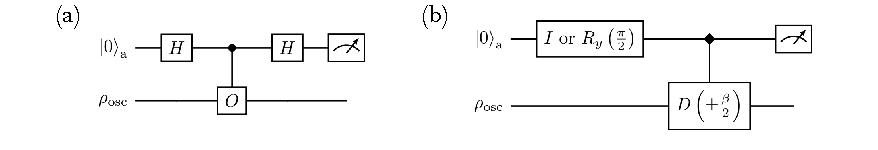
\includegraphics[width=\linewidth]{figures/pdf_figure/ch6/tomography.pdf
        }
    \end{center}
    \caption{
        State tomography for a single mode through measurement of an ancilla
        qubit. (a) The Hadamard test method for measuring the expectation value
        of an arbitrary operator, $\hat O$, applied to the oscillator state,
        utilising an ancilliary qubit. 
        (b) A Hadamard test circuit for measuring the characteristic function, 
        $\chi(\beta)$, of the oscillator using native single qubit rotations and $\sigma_x$-conditioned spin-dependent
        forces (symmetric control represented by the diamond symbol)~\cite{fluhmann_direct_2020}.
        }
    \label{fig:tomography}
    \end{figure}

    With the above methods we may generate interesting non-classical bosonic states, now we
    provide a method for characterising them.\\
    In contrast to a two-level system, the state of an oscillator may not be
    directly readout through state dependent fluorescence. This is due to the much larger state-space of
    the qumode, and the technical difficulty in direct motional readout on the ion-trap platform. To solve these issues, a modular readout scheme is used, involving indirect readout of the oscillator state via a discrete collection of controlled unitaries subject to an ancillary qubit, and computational basis measurements of that ancilla.\\
    The information is mapped to the ancilla by a Hadamard test~\cite{cleve_quantum_1998}, shown in
    figure~\ref{fig:tomography} (a). Here the expectation of observable $\hat O$ on the oscillator, $\langle \hat O\rangle=\mathrm{Tr}(\hat O\rho_\mathrm{osc})$, 
    is recovered through exclusive measurements of the ancilla qubit after qumode-dependent phase ``kick-backs'' are applied. 
    The Hadamard test has the convenient relation between computational basis measurements of the ancilla, and the expectation of the state-under-test observable, $\langle\hat\sigma_z\rangle = \mathrm{Re}\big[\mathrm{Tr}(\hat O\rho_\mathrm{osc})\big]$.\\
    Full state tomography may now be formulated by repeat measurements of the conditional displacement operation, 
    $\hat O = e^{-i\theta}\hat D(\beta)$, to recover the characteristic function, defined as $\chi =
    \mathrm{Tr}(D(\beta)\rho_\mathrm{osc})$, $\beta$ is a complex parameter with displacement magnitude, $|\beta|$, and displacement axis, $\arg(\beta)$.
    Final computational state measurements of the Hadamard test circuit then yield,
    \begin{align}
    \langle \sigma_z \rangle &= \mathrm{Re}\big[e^{-i\theta}\mathrm{Tr}(D(\beta)\rho_\mathrm{osc})\big],\\
                             &= \cos(\theta)\mathrm{Re}[\chi] + \sin(\theta)\mathrm{Im}[\chi],
    \end{align}
    where $\theta$ may be set to $0$ or $\pi/2$ to recover the real or imaginary part of the characteristic function respectively.
    Each measurement provides only 1-bit of information on the (continuous) oscillator state, thus to approximate a useful reconstruction, 
    many samples with a range of $\beta$ values must be collected.\\
    Once the characteristic function has been measure, it can be converted to other familiar representations of the oscillator, such as in the Fock-state basis, or Wigner representation~\cite{wigner_quantum_1932, cahill_density_1969, vogel_determination_1989}. In this work, we shall keep to the conveniently measured characteristic function.\\
    To give two concrete example, the vacuum state characteristic function is the circularly symmetric Gaussian state,
    \begin{equation}
        \chi_\mathrm{0} = \mathrm{exp}\left(\frac{-|\beta|^2}{2}\right),
    \end{equation}
    while the squeezed state, with squeezing parameter $\xi = re^{i\phi}$, breaks this symmetry due to a contraction on one axis, and a corresponding expansion on the other~\cite{lo_spinmotion_2015},
    \begin{equation}
        \label{eqn:sqz_char}
        \chi_\mathrm{S} = \mathrm{exp}\left(\frac{-|\beta|^2}{2}\left(e^{2r}\cos^2(\phi')+e^{-2r}\sin^2(\phi')
        \right)\right),
    \end{equation}
    where $\phi'$ is the angle between squeezing axis and probe axis, $\phi'=\arg(\beta)-\frac{\phi}{2}$.\\

    Experimentally the $\hat\sigma_x$ conditioned spin-dependent force are simply accessed by the bichromatic field method discussed in \S~\ref{sec:SDF}. The Hadamard test circuit is decomposed to native gates, shown in
    figure~\ref{fig:tomography} (b), first described in
    reference~\cite{fluhmann_direct_2020}. The proceeding $I$ or
    $R_y(\pi/2)$ set the quadrature to measure; $\mathrm{Re}(\chi)$ or $\mathrm{Im}(\chi)$
    respectively.
    This circuit provides a practical method for characterising a single qumode,
    which we shall use in the following experimental demonstration. We note,
    similar to the constraints of state characterisation discussed in
    \S~\ref{sec:k-copy_char}, full tomographic reconstruction is
    intractable for multiple-qumodes due to the large state-space, even with
    reasonably truncated oscillator representations (e.g. imposing a Fock-state
    cut-off). In the case of characterising systems consisting of multiple
    qubits and qumodes, either reduced tomography~\cite{he_efficient_2024}, or simplified metrics of performance~\cite{valahu_benchmarking_2024} must be used.
    
\subsection{Experimental Demonstration}
    % - Point to motional coherence time. Was dephasing dominated, improved by grounding \\
    In our group, we have previously demonstrated higher order
    squeezing~\cite{bazavan_squeezing_2024}, superpositions of non-linear
    bosonic states~\cite{saner_generating_2024},
    beam-splitter~\cite{saner_real-time_2025}, and two-mode squeezing
    interactions. However, due to the constraints of the previous experimental
    apparatus we were limited to global addressing fields, preventing the
    application of these hybrid interactions to more than two qubits. Here we
    demonstrate the creation and characterisation of a squeezed state on the
    newly constructed apparatus, described in chapter~\ref{ch:apparatus},
    utilising the single-qubit addressing system. Single addressing both
    increases the power efficiency of the interactions, and allows the control
    to select which qubit is used to couple to the motion --- this provides a
    scalable route to generating hybrid interactions on larger qubit, and qumode
    registers.\\
    
    \begin{figure}
    \begin{center}
    \noindent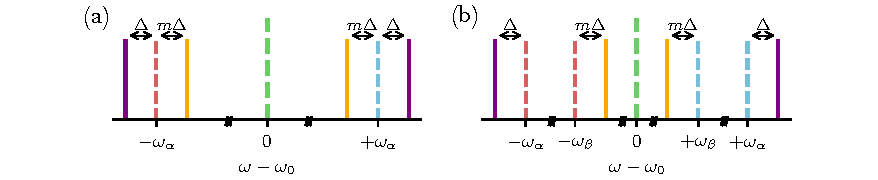
\includegraphics[width=\linewidth]{figures/pdf_figure/ch6/four_tones.pdf
        }
    \end{center}
    \caption{
    The quadchromatic field required for generating non-linear motional interactions via the two-SDF method. (a) For single-mode interactions, both SDF fields are detuned around the sidebands of the same motional mode, $\omega_\alpha$. Integer $m$ is varied to select the desired interaction. (b) For two-mode interactions, each SDF is detuned from a different motional mode.
        }
    \label{fig:2-SDF}
\end{figure}
\subsubsection{Two Spin Dependent Forces}
    The individual SDFs are generated by the same bichromatic field method
    described in \S~\ref{sec:sdf} --- i.e. simultaneous off-resonant blue-
    (BSB) and red-sidebands (RSB) of motional mode $\omega_\alpha$ are applied.
    As such, we require four optical fields with, frequency, phase, and
    amplitude control. The four required frequencies of the ``quadchromatic''
    field are shown schematically in figure~\ref{fig:2-SDF} with respect to the
    carrier frequency, $\omega_0$. Here, purple lines correspond to
    SDF$_\alpha$, and orange lines to SDF$_\beta$. In this example we show the
    SDFs acting on a shared motional mode, but in general they may act on
    different modes. Similar to the generation of the bichromatic field, we may produce this
    quadchromatic field through the application of four RF tones onto a
    single-pass (SP) AOM. These tones are generated using an arbitrary waveform
    generator (AWG)\footnote{\emph{Sinara Phaser} board}. We cannot control the
    absolute optical phase at the ion, however we can set relative phases
    between the four fields by applying phase offsets between the RF tones with
    respect to some fixed time point.
    As discussed in \S~\ref{sec:sdf}, the spin phase of the SDFs is set by
    the absolute phase of the RSB and BSB, $\hat\sigma_\phi =
    \cos(\phi_s)\hat\sigma_x + \sin(\phi_s)\hat\sigma_y$. To ensure we saturate
    the non-commutativity of the spin conditioning of the two SDFs, we require
    $\pi/2$ phase difference between the two spin phases,
    \begin{equation}
        \label{eqn:spin_phase}
        \phi_{\alpha, s} - \phi_{\beta,s} = \frac{\phi_{\alpha,\mathrm{RSB}}+\phi_{\alpha,\mathrm{BSB}}}{2}-\frac{\phi_{\beta,\mathrm{RSB}}+\phi_{\beta,\mathrm{BSB}}}{2}=\frac{\pi}{2}.
    \end{equation}
    In the following demonstration we set $\phi_{\alpha,\mathrm{RSB}}=
    \phi_{\alpha,\mathrm{BSB}}=\pi/2,\phi_{\beta,\mathrm{RSB}}=\phi_{\beta,\mathrm{BSB}}=0$,
    however we note that for composing multiple hybrid operations into a
    circuit, the resulting motional phase of the SDFs can lead to further
    constraints on the chosen RSB and BSB phases.\\
    The intensity of the quadchromatic field is ramped on and off with a rise
    envelope of $\sin^2(\pi t/(2t_\mathrm{ramp}))$ applied via the AWG, where
    $t_\mathrm{ramp}$ is the ramp duration. This ramp suppresses excess off-resonant
    excitations of the $A_1$ phase loop term given in the previous section, and
    so we must select its duration based on the characteristic scale,
    $\frac{1}{\Delta}$. \\
    We aim to balance the power in each of the 4 tones. This may be calibrated
    using an optical pick-off before addressing the ion, directed onto a fast
    photodiode, and measuring the beatnote contrast when applying any pair of
    tones. In the following squeezing demonstration, we balance the tones
    comprising the individual SDFs, but do not explicitly balance the power
    between SDFs, as the desired interaction scales as
    $\Omega_\alpha\Omega_\beta$, any imbalance leads to non-optimal interaction
    efficiency, but unlike imbalance of the RSB and BSB, does not increase
    coherent error terms.
    We observe that the duty cycle of the SP AOM can dramatically shift the
    power imbalance between all four tones, and so we take care ensuring that
    the total RMS power to drive one-, two-, and four-tones is the same as for
    the idle (no optical pulse) setting of the SP AOM, thus the only transient
    power drop is that of the ramp sequence. \\
    

\subsubsection{Squeezing}
    - \todo{potential plot: check ramp is sufficient by looking at $\sigma_z$ dependence. If want ramp have rid 120238, 119279}\\

    We demonstrate the effective squeezing interaction on a single ion and radial
    motional mode. We are limited to using the
    radial modes due to the geometry single addressing system with respect to
    the trap. We use the upper radial mode with frequency,
    $\omega_{upper}=2.87~\unit{\mega\hertz}$, and motional coherence $\tau_\mathrm{upper}=19(1)$\todo{rid 135596} given in
    \S~\ref{sec:motional_coherence}.
    The initial near-vacuum motional state is prepared by Doppler and sideband cooling, with a typical thermal fock state distribution with mean $\bar{n} = 0.03(1)$, as described in \S~\ref{sec:cooling}. The spin state is initialised into the ground state by optical pumping, described in \S~\ref{sec:optical_pump}.
    By setting the relative detuning between the SDFs to $m=-1$, and ensuring anti-commuting spin conditioning by setting the relative phases of the quadchromatic field according to equation~\ref{eqn:spin_phase}, we realise a $\hat\sigma_z-$ conditioned squeezing interaction.
    As the spin-state is prepared in an eigenstate of the spin-conditioned squeezing, we expect squeezing on the qumode, without any change to the qubit state. We use a total quadchromatic beam power of $53~\unit{\micro\watt}$, and set the base detuning, $\Delta=2\pi~50~\unit{\kilo\hertz}$. We suppress excess excitation of the off-resonant error terms by using a ramp of $t_\mathrm{ramp}=40~\unit{\micro\second}$.\\
    The state is characterised by the tomography method given in
    \S~\ref{sec:tomography}, with a discretization set to collect a $35\times 35$ grid of displacement
    values, $\beta$, and $N = 300$ repeat samples to reduce shot noise. The full dataset for one of the tomographic scans takes around 1 hour to collect, and so we interleave mode calibration experiments (\S~\ref{sec:tickle}) to run every 5 minutes.\\
    The on-resonance splitting SDF used for tomography must have its strength, $\Omega_\mathrm{SDF}$, calibrated to infer the magnitude of $\beta$ applied. We use
    a total bichromatic beam power of $40~\unit{\micro\watt}$, and through fitting the 
    $\hat\sigma_z$ expectation for the time-dependent splitting of a vacuum state,
    \begin{equation}
        \langle \hat\sigma_z \rangle = e^{-2|\beta|^2},
    \end{equation}
    with 
    \begin{equation}
        |\beta| = \frac{\Omega_\mathrm{split}t}{2}.
    \end{equation}
    We find $\Omega_\mathrm{split}=2\pi~7.2(4)~\unit{\kilo\hertz}$. \\
\begin{figure}
    \begin{center}
    \noindent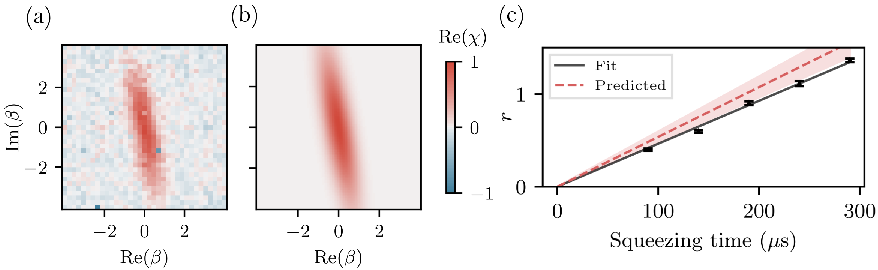
\includegraphics[width=\linewidth]{figures/pdf_figure/ch6/sqz_data.pdf
        }
    \end{center}
    \caption{
        Demonstration of the squeezing interaction through the two-SDF method. (a) The characteristic function, $\mathrm{Re}\left(\chi\left(\beta\right)\right)$, of the squeezed state measured using the state tomography method given by figure~\ref{fig:tomography}. (b) The simulated state taking fit parameters inferred by equation~\ref{eqn:sqz_char}. (c) The fitted squeezing parameter, $r$, as a function of two-SDF pulse duration.
        }
    \label{fig:squeezing}
\end{figure}
    The pulse sequence for squeeze state generation and characterisation is
    given in figure~\ref{fig:squeeze_pulses}, and the resulting real part of the
    characteristic function is shown in figure~\ref{fig:squeezing} (a).
    Fitting the data to equation~\ref{eqn:sqz_char} we may extract both the
    squeezing axis, $\phi$, and the strength, $r$, where $r$ is given by,
    \begin{equation}
    r=|\Omega_\mathrm{eff,S}|t=\frac{\Omega_\alpha\Omega_\beta}{2}t.
    \end{equation}
    An example fit is shown in
    panel (b), with extracted $r=0.90(2)$, for a quadchromatic FWHM pulse
    duration of $t_\mathrm{sqz}=190~\unit{\micro\second}$. Panel (c) displays
    the squeezing strength as a function of $t_\mathrm{sqz}$, with fit values given by the points, and the black line is a linear fit. Assuming that the two SDF strengths are well balanced, $\Omega_\alpha=\Omega_\beta$, and taking the $53~\unit{\micro\watt}$ used for the quadchromatic field compared to the SDF strength calibration at $40~\unit{\micro\watt}$, we find an expected squeezing strength of $\Omega_\mathrm{eff,S} = 2\pi~0.86(9)~\unit{\kilo\hertz}$. This is shown as the red dashed line and shaded region.
    The fitted strength of $\Omega_\mathrm{eff,S}= 2\pi~0.74(1)~\unit{\kilo\hertz}$ is lower than the expected, suggesting that either we are not sufficiently balancing the strengths of the two simultaneous SDFs, or that the power stabilisation routine for 4-tones is inaccurate. Further exploration is needed, including careful quantification of the individual SDF strengths constituting the quadchromatic field. However, this preliminary result confirms that the motional coherence, and stability of the single-addressing system is sufficient to create, and characterise non-classical motional states using the apparatus developed for this thesis.\\
    \todo{Comment on heating rate}

\subsection{Outlook}
    Hybrid systems offer access to large Hilbert spaces, even with modest ion numbers.
    In this section we outlined a convenient set of native interactions for universal hybrid qubit-qumode gates. We experimentally demonstrate the squeezing interaction generated via the ``two-SDF'' method of
    reference~\cite{sutherland_universal_2021}. This demonstration replicated previous work using the ``two-SDF'' method~\cite{bazavan_squeezing_2024}, however now shown on the newly built apparatus utilising a single-ion addressing system, and applied to the radial motional modes.\\ 
    Enabled by the single-addressing, and improved motional coherence times of
    the new system, we are particularly interested in exploring short hybrid
    circuits composed of multiple interactions acting on an array of qubits and
    qumodes. Specifically, we are interested in utilising the hybrid system with
    increased robustness against errors through the use of quantum error mitigation methods applicable to both 
    spin and oscillator subsystems. We outline one such method in the next section, with a preliminary demonstration on the spin subsystem.\\
    \subsubsection{Limitations}
    Using a single multi-ion chain to access multiple qubits and qumodes for
    scaling hybrid QC on the trapped-ion platform will be ultimately limited by
    spectral crowding of the motional modes, i.e. the average frequency spacing
    between neighbouring modes decreases as the number of accessible modes
    increases. \\
    The ``two-SDF'' method requires frequency selectivity to drive bosonic
    interactions exclusively on the chosen mode. 
    To selectively drive a single mode, the magnitude of the detuning $\Delta$ must follow $\Delta \ll \delta\omega$, where $\delta\omega$ is the frequency difference to the nearest neighbouring mode. As discussed in the ``two-SDF'' method section, the strength of each SDF must be less than the base detuning, $\Omega_\alpha \ll \Delta$, to well approximate the effective non-linear unitary dynamics. As a result of these two requirements, the
    mode-frequency splitting directly limits the attainable strength of the non-linear interaction in the adiabatic regime, resulting in increasing gate duration with increasing register size.\\
    A possible mitigation
    would be to rather scale the hybrid system using a collection of fixed-length
    chains with adequate mode-frequency splitting, and to transport quantum
    information between these chains either through ion transport whilst maintaining mode and spin coherence~\cite{walther_controlling_2012}, generating remote entanglement through photonic interconnects~\cite{luo_protocols_2009}, or through inducing collective motional interactions
    between separate ion-chains~\cite{valentini_demonstration_2025}. \\
    Another
    mitigation strategy could come from the pulse-shaping approach demonstrated
    for use in fast two-qubit entangling gates in the non-adiabatic
    regime~\cite{schafer_fast_2018}, i.e. when $\Delta > \delta\omega$.
    Introducing extra degrees of freedom in the pulse amplitude envelope could allow for
    driving the desired interaction on the selected modes, while returning all spectator modes to their initial state by the end of the pulse. However, we note that the accumulation of
    non-global geometric phases, and possible non-commutativity of interactions
    on shared qubit-oscillator states could prohibit the use of such a
    pulse-shaping scheme. Ultimately, the desired interaction, mode frequency spectra, and target gate duration will determine the dominant coherent errors. We leave such an analysis for future work. \\

\section{\textbf{Virtual Distillation}}
\label{sec:virtual_distillation}
- Motivation for applying QEM on our system. \\
    - For NISQ era, pre FTQC, still methods to improve viability. \\
- In our use case, we are interested in: few required resources, and need compatibility with DV and CV systems. Particularly without need to discretize our oscillator, like e.g. GKP. \\
- Summary of what we will discuss in this chapter, highlighting preliminary results on DV subsystem.\\

Here we develop experimental tools for demonstrating VD on the discrete variable portion of the full hybrid system.
\subsection{Error Mitigation}
\label{sec:QEM}
Noise coupled to a quantum system results in unintended coherent, and incoherent
evolution. Deviations of the realised state from the target state are known as
errors, and, if left unchecked, lead to the failure of quantum algorithms. 
This failure can either be due to a reduction of signal to noise ratio, or a
bias in the measured expectation value, resulting in misleading conclusions. 
Ultimately, the goal of quantum error correction, QEC, is to detect and correct
these errors through embedding information in a larger Hilbert space~\cite{qec_review}.
Full QEC will allow for the execution of arbitrarily long algorithms ensuring errors (of
up to a certain distance) do not accumulate over time. However, current QEC
methods require large overheads in both qubit number and circuit depth, and are
therefore not feasible on current quantum hardware. Furthermore, QEC is
formulated for digital ``gate-based'' quantum computers, which although promise
to be universal, pay for that privilege in often inefficient decompositions of
target unitaries into a discrete set of gates. 
This poses an opportunity for
near term devices to show quantum advantage using either short depth,
uncorrected circuits, or analog quantum simulators, which although not
universal, can provide meaningful results for specific problems~\cite{nisq_review}. Particularly,
phrasing the problem in terms of expectation values of an observable on a
physical final state, rather than a sequence of measurements on a set of logical
state, allows for a more efficient use of resources. As a tactile example,
consider the problem of finding the ground state energy of a Hamiltonian. This
can be done by preparing a trial state, and directly measuring the expectation
value of the Hamiltonian on that state, building up statistics over many
samples~\cite{variational_qc_review}. Increasing the number of samples will reduce the statistical error,
however, if the trial state is not prepared perfectly due to either
environmental noise, or to imperfect application of unitary evolutions, the
measured expectation value will be biased. 
To this end, quantum error
mitigation (QEM) techniques have been developed to reduce the bias of measured
expectation value of an observable at the expense of requiring more samples. 
Reference~\cite{cai_quantum_2023} defines QEM as
``... algorithmic schemes that reduce the noise-induced bias in the expectation value by postprocessing outputs from an ensemble of circuit runs, using circuits at the same noise level as the original unmitigated circuit or above.''
This highlights the crux of how information on the system is collected by a QEM implementation, which I shall explore with the following thought experiment on the ``perfect'' QEM algorithm.\\
\begin{figure}
    \begin{center}
    \noindent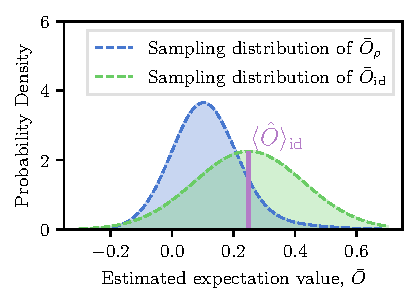
\includegraphics[width=0.5\linewidth]{figures/pdf_figure/ch6/qem_schem.pdf
        }
    \end{center}
    \caption{
    \todo{ Integrate figure into main text.}
    $\rho = 0.1\rho_\mathrm{id}+0.9 \rho_\mathrm{err}$. Blue curve is PDF for $N$ shots, green is PDF for ideal shots, with $N_\mathrm{id} = 0.1N$.\\
    A schematic explanation of the goal of quantum error mitigation. Deviations of the measured expectation value of an observable $\hat O$ on a noisy state, $\rho$, and on the ideal state $\rho_\mathrm{id}$ may be separated into components originating from shot noise, and from an underlying bias. Shot noise sets the variance of the distribution of estimated expectation values, while the underlying bias shifts the center of the distribution. Error mitigation reduces bias at the cost of increasing variance. Here we demonstrate this by the ideal QEM method introduced in \S~\ref{sec:QEM}. The underlying noisy state is given by $\rho = (1-p)\rho_\mathrm{id} + p\rho_\mathrm{err}$. $N$ shots are taken measuring $\mathrm{Tr}(\hat O \rho)$. The ideal QEM flags and discards shots originating from $\rho_\mathrm{err}$, leaving $(1-p)N$ shots of the ideal state to estimate $\langle \hat O \rangle$.
        }
    \label{fig:qem}
\end{figure}

Consider the problem of measuring the expectation value of an observable $\hat{O}$ on the target state $\rho_{id}$. The state is prepared by a quantum circuit, which due to noise, instead prepares the mixed state $\rho = (1-\lambda) \rho_{id} + \lambda \rho_{err}$, where $\rho_{err}$ is the error state. Each measurement of the observable $\hat{O}$ on the noisy state $\rho$ will return a value $o_i$, and the average of these measurements will converge to the expectation value $\langle \hat{O} \rangle = \mathrm{Tr}[\hat{O}\rho]$. Given $S$ total samples, the final result will be,
$$ \langle \hat{O} \rangle = \frac{1}{S} \left(\sum_{i=1}^{S_{id}} o_i + \sum_{j=1}^{S_{err}} o_j\right),$$
where $S_{id}$ and $S_{err}$ are the number of samples that return a measurement outcome from the ideal and error states respectively, with $S = S_{id} + S_{err}$. The bias in the measured expectation value from the ideal is then given by contributions from the samples $S_{err}$. An ideal QEM algorithm would flag these error samples, and remove them from the final average, resulting in a bias free expectation value using the restricted samples $S_{id}$.\\
- Finish argument about ideal QEM \\
- Summary of QEM method types (quick overview) and transfer sentence to VD purity type approach. \\
- Why VD:\\
    - operates on noisy physical states rather than requiring logical encoding;\\
    - is applicable to general Hilbert spaces, i.e. hybrid good \\
    - exchanges additional copies/sampling/circuit resources for reduced bias with fixed length (given copy and register size) derangement and measure at end\\
    - is therefore interesting for the multi-register and eventually hybrid architecture considered here.\\

\subsection{Virtual Distillation Protocol}
\label{sec:vir_dist_theory}
- Quick description of goal of purification method (first line of theory), and any particular merit of method e.g. very weak constraints on noise type, highlight we explore one of the failure cases in exp demo.\\
- We will present some background theory on VD, to rationalise the action of the circuit decomposition, taken from references...\\
- We present with exp demo on minimal DV system of two-copies. \\
- And propose future extensions to the hybrid system. \\

\subsubsection{Theory}
\todo{This is rough notes. Be selective of what to present, rationalising by: 1) understanding action of applied circuit, 2) requirement for understanding experimental demo.}\\
- narrative should be how we go from $\rho \rightarrow \rho^k/\rm{Tr}(\rho^k)$ \\
- Followed by when this fails \\
Estimate expectation value of observable on a state without ever physically preparing the state.
Purification here refers to approaching the dominant pure state of a mixed state. The $k$th degree purified state is given by,
\begin{equation}
    \rho_\mathrm{corrected}^{(k)}=\frac{\rho^k}{\mathrm{Tr}[\rho^k]}=\sum_{i=1}^{d} \frac{\lambda_i }{\sum_{i=1}^d \lambda_i^k} \ket{\psi_i}\bra{\psi_i},
\end{equation}
where $d$ is the dimension of the Hilbert space, $\lambda_i$ are the eigenvalues of $\rho$, and $\ket{\psi_i}$ are the corresponding eigenvectors. If we assume that one eigenvalue is dominant, $\lambda_1 \gg \lambda_{i>1}$, then the normalised purified state exponentially approaches the dominant eigenvector, $\rho_\mathrm{corrected}^{(k)} \to \ket{\psi_1}\bra{\psi_1}$, as $k$ increases.
The hope, which we shall verify in section XX on coherent mismatch, is that the dominant eigenvector of the noisy state closely approximates the ideal state, and therefore effective meaurements on the purified state yield accurate expectation values of the ideal state.
The estimated expectation value of measuring an observable, $\hat{O}$, on this purified state is then,
\begin{equation}
    \langle\hat{O}\rangle_\mathrm{corrected}=\mathrm{Tr}[\hat{O}\rho_\mathrm{corrected}^{(k)}]=\frac{\mathrm{Tr}[\hat{O}\rho^k]}{\mathrm{Tr}[\rho^k]}.
\end{equation}
Next, how to access this corrected state on which to make these measurements? Kozcor and Huggins show that this can be accessed without explicit preparation of the purified state. Instead the numerator and denominator may be found through preparing $k$ copies of the noisy state, applying some derangement operation to entangle all copies together, and measuring the desired observable on one of the copies. This can be understood through the following identity,
\begin{equation}
    \mathrm{Tr}[\hat{O}\rho^k]=\mathrm{Tr}[\hat{O}^iS^{(k)}\rho^{\otimes k}],
\end{equation}
where $S^{(k)}$ is the derangement operator, which permutes the $k$ copies of the state, and $\hat{O}^i$ is the observable acting on the $i$th copy. We shall define the derangement operator explicitly as the cyclic permutation of $k$ objects,
\begin{equation}
    S^{(k)}\ket{\psi_1}\otimes\ket{\psi_2}\otimes...\otimes\ket{\psi_k}=\ket{\psi_2}\ket{\psi_3}\otimes...\otimes\ket{\psi_k}\otimes\ket{\psi_1}.
\end{equation}
\todo{Move following to appendix, or cut.}\\
Huggins provides a proof of this identity, which I reproduce here for the simple example of $k=2$.   The derangement operator for two copies is simply the swap operator, $S^{(2)}=\mathrm{SWAP}$, and we will assume the observable acts only on the first copy, giving $\hat{O}^1 = \hat{O}\otimes\mathbb{I}$. The identity is then,
\begin{align}
    \mathrm{Tr}[\hat{O}^1S^{(2)}\rho^{\otimes 2}]&\\
    &= \sum_{\substack{i_1,i_2\\j_1,j_2\\k_1,k_2}} \bra{i_1}\hat{O}\ket{k_1}\delta_{i_2,k_2}
    \bra{k_1, k_2}S^{(2)}\ket{j_1,j_2}\bra{j_1}\rho\ket{i_1}\bra{j_2}\rho\ket{i_2}\\
    &= \sum_{\substack{i_1,i_2\\j_1,j_2\\k_1, k_2}} \hat{O}_{i_1, k_1}\delta_{i_2,k_2}\delta_{k_1,j_2}\delta_{k_2,j_1}\rho_{j_1,i_1}\rho_{j_2,i_2}
\end{align}
and contracting the Kronecker deltas, we find,
\begin{align}
    \mathrm{Tr}[\hat{O}^1S^{(2)}\rho^{\otimes 2}]&\\
    &= \sum_{\substack{i_1,j_1, j_1}} \hat{O}_{i_1, j_2}\rho_{j_1,i_1}\rho_{j_2,j_1}\\
    &= \mathrm{Tr}[\hat{O}\rho^2],
\end{align}
with the last equality following from the definition of matrix multiplication. \\
\todo{======================================================}\\
The denominator of the corrected expectation value is found by replacing the observable with the identity and measuring the expectation value of the derangement operator on $k$ copies of the noisy state.\\
Access to this corrected expectation value is then possible if we can measure the multi-qubit observable $\hat{O}^iS^{(k)}$ on $k$ copies of the noisy state. \\

Next, need to derive scaling of bias with copy number. And finally, discuss the variance of measurement with shot number (and how this scales with copy number?).

\subsubsection{Circuit}
\begin{figure}
    \begin{center}
    \noindent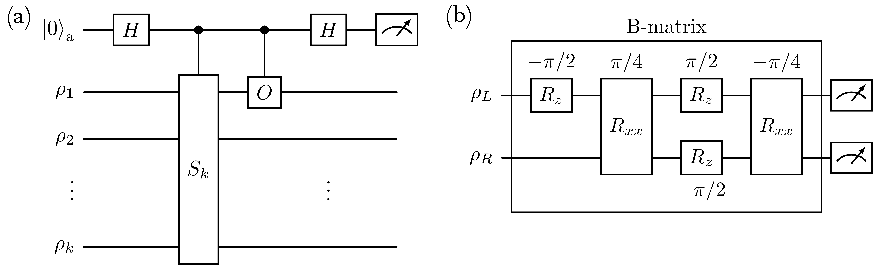
\includegraphics[width=1.0\linewidth]{figures/pdf_figure/ch6/virdist_circuits.pdf
        }
    \end{center}
    \caption{
        \todo{Figure: circuit diagram for ancilla based virtual distillation, Hadamard test, derangement operator by CSwap}\\
        \todo{Update B circ to pi/4 gates}\\
        Two circuits for implementing virtual distillation. (a) Hadamard test method using controlled derangement, $S_k$, over $k$ copies, and controlled observable, $\hat O$, applied on one copy. The ancilla qubit is measured to extract $\mathrm{Tr}(\hat O\rho^k)$. Repeating the circuit without the controlled observable measures normalisation factor, $\mathrm{Tr}(\rho^k)$, used to recover the virtually purified result, $\langle \hat O\rangle_\mathrm{VD}$. (b) Two-copy implementation using a $B$-circuit, here decomposed into two entangling gates and single qubit phase gates. Measurement of both qubits in the computational basis, and classical postprocessing recovers $\mathrm{Tr}(Z\rho^2)$ and purity, $\mathrm{Tr}(\rho^2)$, used to recover $\langle Z \rangle_\mathrm{VD}$.
        }
    \label{fig:virdist_circuit}
\end{figure}
- We present two possible physical implementations of VD. The first being a scalable strategy based on Hadamard test with ancilla, second being resource efficient but limited to XXX check flow chart in Huggins.\\
    - Present ancilla method, describing circuit and maybe give intuition on phase kick back to ancilla?\\
    - B-matrix protocol, if we diagonalise both S and SO, no need for ancilla and we get purity and TrO immediately. \\

We will discuss two methods of implementing this measurement. First, a Hadamard test, given in Fig.~\ref{fig:hadamard_test}, which uses an ancilla qubit to control the derangement and desired observable operation, and then subsequent measurement of the ancilla only. The second method, given in Fig.~\ref{fig:b_matrix}, uses a B-matrix to implement the derangement operation, and then measures the observable on one of the copies. 
The Hadamard test is more general, as it can be used to measure any observable, however, it requires an additional ancilla qubit and controlled operations. The B-matrix method has better qubit number and operation depth efficiency, however, requires simultaneous diagonalisation of $S^{(k)}$ and $\hat{O}^iS^{(k)}$, which is not always possible for an arbitrary observable and derangement operator.

% \subsubsection{Noise Floor}
% \begin{itemize}
%     \item Discuss noisefloor (coherent mismatch)
%     \item Go into detail on how spatially correlated noise can be an issue here, discuss network paper as opposite case
% \end{itemize}
% \todo{Figure: Simulation of vir dist on various noise models.}

% Comparing to bias reduction with copy number, describe that this exponential reduction cannot hold indefinitely for arbitrary noise models, and that there is a noise floor. For a single qubit with depolarising noise, there is no such floor, however we note the effect of coherent mismatch, which for copys consisting of multiple qubits, even depol noise leads to coherent drift.
% Furthermore, we are particularly interested in the effect of correlated noise on the separate registers leading to irremovable errors. Correlated noise, as discussed in chapter 5, can dominate the error budget when copies are stored in similar physical locations, and within shared noisy fields. The practical mitigation for this is to separate the copies in space and environment, e.g. over a network (tenzan paper), or to decorrelate errors through local randomisation (randomised compiling, twirling, etc). We shall explore the effect of correlated noise on virtual distillation practically in section x. But first, here we show an analytic model of the effect of correlated noise on a small two-copy system.
% Describe model of k-copy clifford noise, likening it to a deep random circuit ran in parallel on each copy. This is the same noise channel enforced through k-copy twirling. As with chapter 5, this gives us a natural language of irreps to describe the action of our noise channel on an initial state. We may describe the B matrix in this irrep basis, and show the final populations of the copies after derangment. Finally, taking the <Z> measurements on both copies, we can recover the corrected expectation value of the observable. To conform with RB type decay curves, we show the decay of the corrected expectation value with number of Cliffords. We note that another view of this data, more common in error mitigation literature, is a plot of error suppression versus total error ?lambda. From chapter 5 we now that the uncorrected single qubit decay is given by,
% \begin{equation}
%     \langle Z \rangle_\mathrm{uncorrected} = (1-\varepsilon_{dp}-\varepsilon_{corr})^m,
% \end{equation}
% where $\varepsilon_{dp}$ is the depolarising error rate, $\varepsilon_{corr}$ is the correlated error rate, and $m$ is the number of Cliffords applied. This is plotted as dashed line.
% The corrected expectation value is given by $<Z>_{corrected}$ in the presence of both depolarising and correlated noise.
% We can see from the figure that under dominant depolarising noise we see a large suppression of error, however, under dominant correlated noise, the error is largely unaffected. Analytically we find that the final decay of the corrected expectation value is given by,
% \begin{equation}
%     \langle Z \rangle_\mathrm{corrected} = \frac{2\left(\left(1-\varepsilon_{corr}\right)\left(1-\varepsilon_{dp}\right)\right)^m}{1+\left(1-\varepsilon_{dp}\right)^{2m}},
% \end{equation}
% We see that for $\varepsilon_{corr} = 0$, we recover the expected exponential suppression of error with copy number, however, for $\varepsilon_{corr} > 0$, we find a noise floor in the corrected expectation value.
% Extend this analysis to copy number $k$. Currently, I get here through Liouville form, is there a way to go directly from symmetry on the states?

\subsection{Experimental Demonstration}
- First: establish that you can implement VD: implementation, calibration for minimal demo.\\
- Second: use it to answer a scientific question: Injection of correlated noise \\

\begin{figure}
    \begin{center}
    \noindent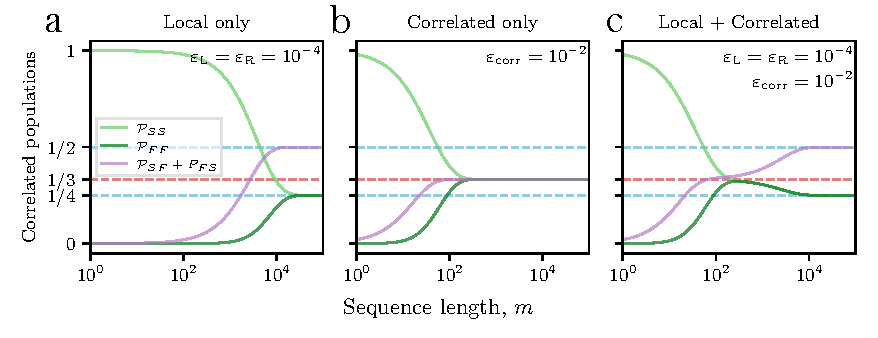
\includegraphics[width=\linewidth]{figures/pdf_figure/ch4/asymptote.pdf
        }
    \end{center}
    \caption{
    \todo{Figure: pi-4 MS gate calibration}. 
    \todo{Figure: Heuristic signal of B-matrix working}. 
    \todo{Tomography would be best!}
        }
    \label{fig:bmatrix_calib}
\end{figure}
\subsubsection{Virtual Distillation on Two Copies}
- Minimal demo is two single qubits. \\
- B circuit demo, consisting of pi-4 gates.\\
- For single qubit phase push, we use single addressing, push phase on AOD. \\
- pi/4 gates are walsh 1, calibrated through applying two consecutive and applying same protocol as described in characterisation.\\
- Give exact numbers for pi/4 gates: loops, power, detuning, duration, fidelity, ramp duration. \\
- B circuit phases were checked using heuristic method, applying differential single qubit rotation to each. \\
- Mention here that tomography would have been better? \\
\begin{figure}
    \begin{center}
    \noindent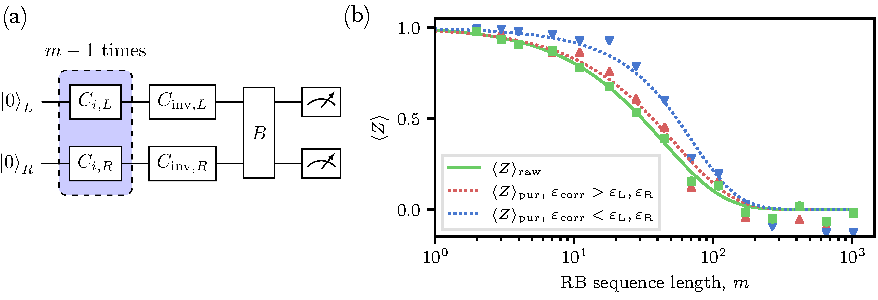
\includegraphics[width=\linewidth]{figures/pdf_figure/ch6/noise_injection.pdf
        }
    \end{center}
    \caption{
        \todo{Figure: Cicruit diagram of RB + VD, exp data for noise floor for two copy B-matrix, with and without spatial correlations}\\
        Verifying the performance of virtual distillation under either dominant local depolarising or correlated errors. Structured errors were injected through a fixed frequency detuning of the 729-nm laser, and the application of a sequence of random Clifford gates. In the case that identical Clifford gates, $C_{i,L} = C_{i,R}$, are applied on both qubits, the detuning error is twirled to a \emph{common noise} channel, while in the case that Clifford gates are sampled independently for both copies, the detuning is twirled to local depolarisation channels. The local and correlated injected error-per-Clifford for both regimes are quantified using \emph{k-copy} RB. Panel (a) shows the circuit of injected errors followed by the $B$-circuit. Panel (b) shows the effective reduction in error-per-Clifford by applying the virtual distillation circuit. The green points correspond to the raw single-qubit decay due to the physical errors, the solid green line is a fit of this decay to measure a total error-per-Clifford. The red and blue points correspond to the error mitigated $Z$ observables for the dominant correlated errors and local depolarising errors respectively. The dotted lines correspond to the expected error mitigated single qubit decays inferred by the model given in equation~\ref{eqn:vd_correlated}, and the error-per-Cliffords measured by \emph{k-copy} RB.
               }
    \label{fig:bmatrix_injection}
\end{figure}
\subsubsection{Virtual Distillation under Correlated Errors}
- We target demo of suppression, of controlled injected errors, that are quantified by k-copy RB. \\
- Give explicit form for suppression of correlated and uncorrelated channels. Look at IRO presentation\\
- Mention this is found by B circuit applied in Pauli basis and using eqn kcopy pops\\
- Give motivation of why k-copy RB is particularly relevant to untwirled VD\\
- Present data in form of single qubit decay rates.\\
- Give analysis and fits. \\

\subsection{Outlook}
- Summary of what we have shown experimentally so far.\\
- Linker sentence to next experimental steps. \\
\subsubsection{Extending to $>2$ copies}
    - plan for controlled swap implementation, requirements for this. \\
    - How many gates, what fidelity we need to ensure tot-err $<1$ for derangement side. \\
    - Given 98\% how many copies could we go to? Can we estimate shot numbers here? Summary in a table would be nice. \\
    - copy number | derangement gates | circuit fidelity | expected sampling overhead\\

\subsubsection{Virtual Distillation on Hybrid Systems}
    - Why important to develop, applications in simulations of QO demo, Feynman, gauge theories. \\
    - Cite Quantum virtual cooling\\
    - How it looks on a thermal state and on various quantum states (sqz, coherent, fock)\\
    - How we can implement c-swap using CV gate set. \\

\subsubsection{Limitations} 
    - Never actually remove entropy from system, so we are limited to total error rate $<1$, unlike QEC. This places us firmly in NISQ applications.\\
    - Coherent and structured errors. Mitigation is twirling.\\
    - Coherent noise floor \\
    - Slow readout if mapping to single ancilla?\\

\begin{figure}
    \begin{center}
    \noindent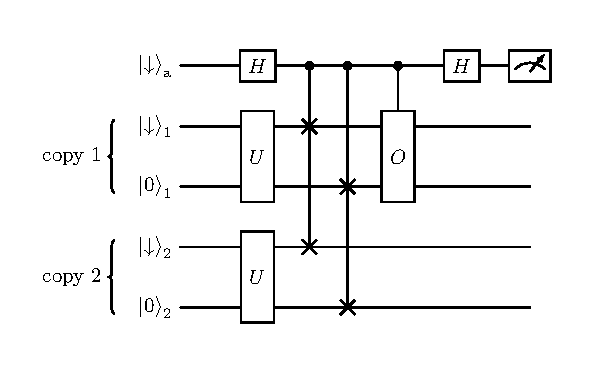
\includegraphics[width=0.7\linewidth]{figures/make_figure/ch6/circs/fredkin/circuits.pdf
        }
    \end{center}
    \caption{
        \todo{Figure: Fredkin gate on oscillator, and how to compose derangement transversally.}.
        Proposed circuit for applying virtual distillation to a hybrid system. Using the ancilla method for measuring $\mathrm{Tr}(\hat O \rho^k)$, we may decompose the controlled derangement to the transversal application of Fredkin gates. 
        }
    \label{fig:fredkin}
\end{figure}
% \begin{figure}
%     \begin{center}
%     \noindent
\includegraphics[width=\linewidth]{figures/pdf_figure/ch4/asymptote.pdf
%         }
%     \end{center}
%     \caption{
%     \todo{Figure: Simulation of tri-sqz state with VD to show negativity!}
%         }
%     \label{fig:virdist_sim}
% \end{figure}

\section{Conclusions}
\todo{
- Summary of chapter, saying this gives our future directions.\\
- Future planned hardware extensions will give more options for CV. Standing wave extension}\\
